\section{Schließende Statistik}
\label{sec:schliessende_statistik}
\subsection{Zufallsstichproben}
\label{sec:zufallsstichproben}
Eine einfache Zufallsstichprobe vom Umfang $n$ ist eine Folge von stochastisch unabhängigen und identisch verteilten Zufallsvariablen
$X_1, \ldots, X_n$, den sogenannten Stichprobenvariablen. Dabei bezeichnet $X_i$ die Merkmalsausprägung des $i$-ten Elements in der Stichprobe.
Die beobachteten Merkmalswerte $x_1,\dots,x_n$ der $n$ Elemente sind Realisierungen der Zufallsvariablen $X_1,\dots,X_n$ und heissen Stichprobenwerte.
\subsection{Parameterschätzungen}
\label{sec:parameterschaetzungen}
Allgemein ist eine Stichprobenfunktion eine Funktion, die von den Stichprobenvariablen $X_1, \ldots, X_n$ abhängt. 
Eine Schätzfunktion $\Theta = g(X_1, \ldots, X_n)$ ist eine spezielle Stichprobenfunktion, nämlich eine „Formel“, mit der man den Wert eines Parameters
$\Theta$ der Grundgesamtheit schätzen kann: Setzt man eine konkrete Stichprobe $x_1, \dots, x_n$ ein, so erhält man einen Schätzwert 
$\hat{\Theta} = g(x_1, \dots, x_n)$ für den unbekannten Parameter $\theta$.
\subsubsection{Erwartungstreue und Konsistente Schätzfunktionen}
\label{sec:erwartungstreue_schaetzfunktionen}
Eine Schätzfunktion $\Theta$ eines Parameters $\theta$ heisst erwartungstreu, wenn gilt:
\begin{equation*}
    E(\Theta) = \theta
\end{equation*}
Gegeben sind zwei erwartungstreue Schätzfunktionen $\Theta_1$ und $\Theta_2$ eines Parameters $\theta$. Man nennt $\Theta_1$ effizienter als $\Theta_2$, wenn gilt:
\begin{equation*}
    V(\Theta_1) < V(\Theta_2)
\end{equation*}
Eine Schätzfunktion $\Theta$ eines Parameters $\theta$ heisst konsistent, wenn gilt:
\begin{equation*}
    E(\Theta) \rightarrow \theta \quad \text{und} \quad V(\Theta) \rightarrow 0 \quad \text{für} \quad n \rightarrow \infty
\end{equation*}
\subsection{Schätzfunktionen für die wichtigsten statistischen Parameter}
\label{sec:schaetzfunktionen_fuer_die_wichtigsten_statistischen_parameter}
\begin{center}
    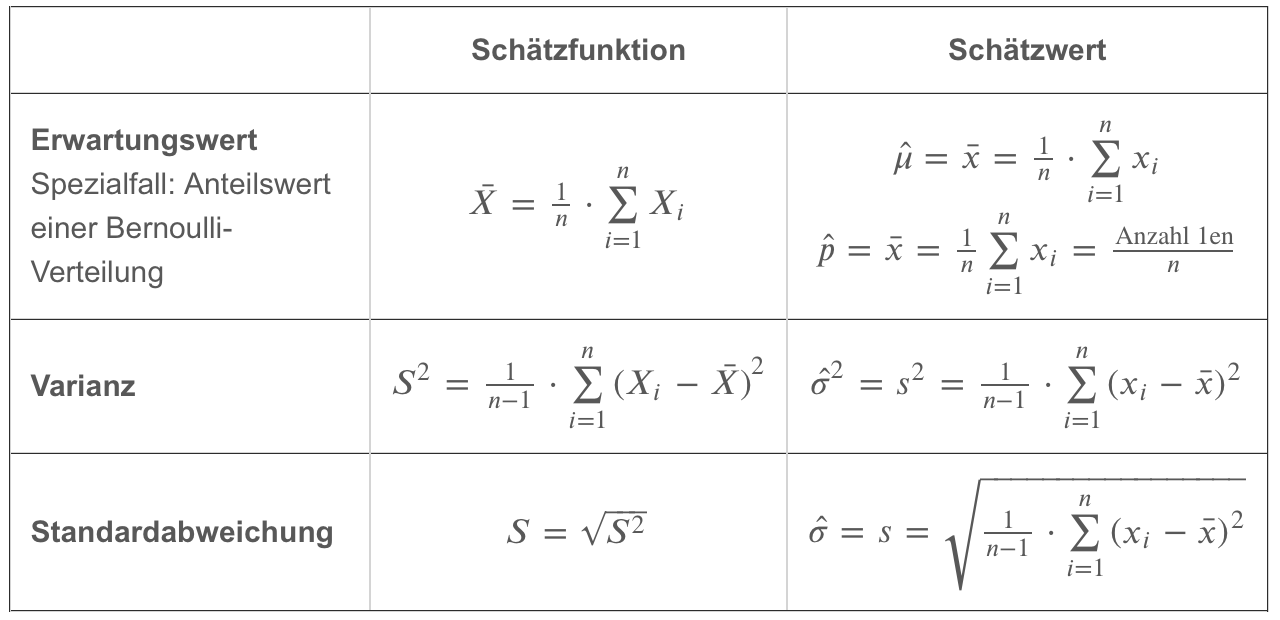
\includegraphics[width=1\linewidth]{images/schaetzfunktionen}
    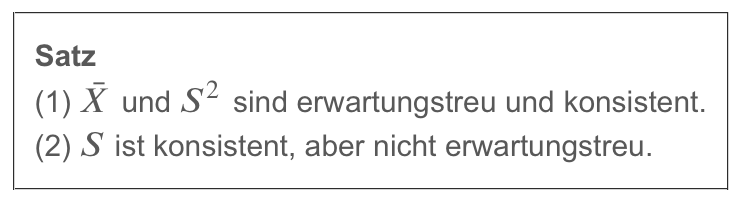
\includegraphics[width=0.5\linewidth]{images/schaetzfunktionen2}
\end{center}
\subsection{Vertrauensintervalle}
\label{sec:vertrauensintervalle}
Man bestimmt zwei Stichprobenfunktionen $\Theta_u$ und $\Theta_o$, die den wahren Wert des Parameters $\theta$ mit der vorgegebenen Wahrscheinlichkeit
$\gamma$ einschliessen: 
\begin{equation*}
    P(\Theta_u \leq \theta \leq \Theta_o) = \gamma
\end{equation*}
Setzt man nun die Werte $x_1,x_2,\dots,x_n$ einer konkreten Stichprobe in $\Theta_u$ und $\Theta_o$ ein, so erhält man die Zahlen $c_u$ und $c_o$.
Das Intervall $[c_u,c_o]$ heisst Vertrauensintervall für den unbekannten Parameter $\theta$. \\
Die Wahrscheinlichkeit $\gamma$ heisst Vertrauensniveau oder statistische Sicherheit (übliche Werte: 95\% oder 99\%);
$\alpha = 1 - \gamma$ wird Irrtumswahrscheinlichkeit genannt. \\
Wenn man hundertmal eine Stichprobe nehmen und zu jeder Stichprobe das Vertrauensintervall berechnen würde, so würden etwa $100 \cdot \gamma$
dieser Intervalle (bei $\gamma = 95\%$ also etwa $95$) den wahren Wert des Parameters $\theta$ enthalten. \\
\subsection{Übersicht über verschiedene Vertrauensintervalle zum Niveau $\gamma$}
\label{sec:uebersicht_ueber_verschiedene_vertrauensintervalle_zum_niveau_gamma}
\begin{center}
    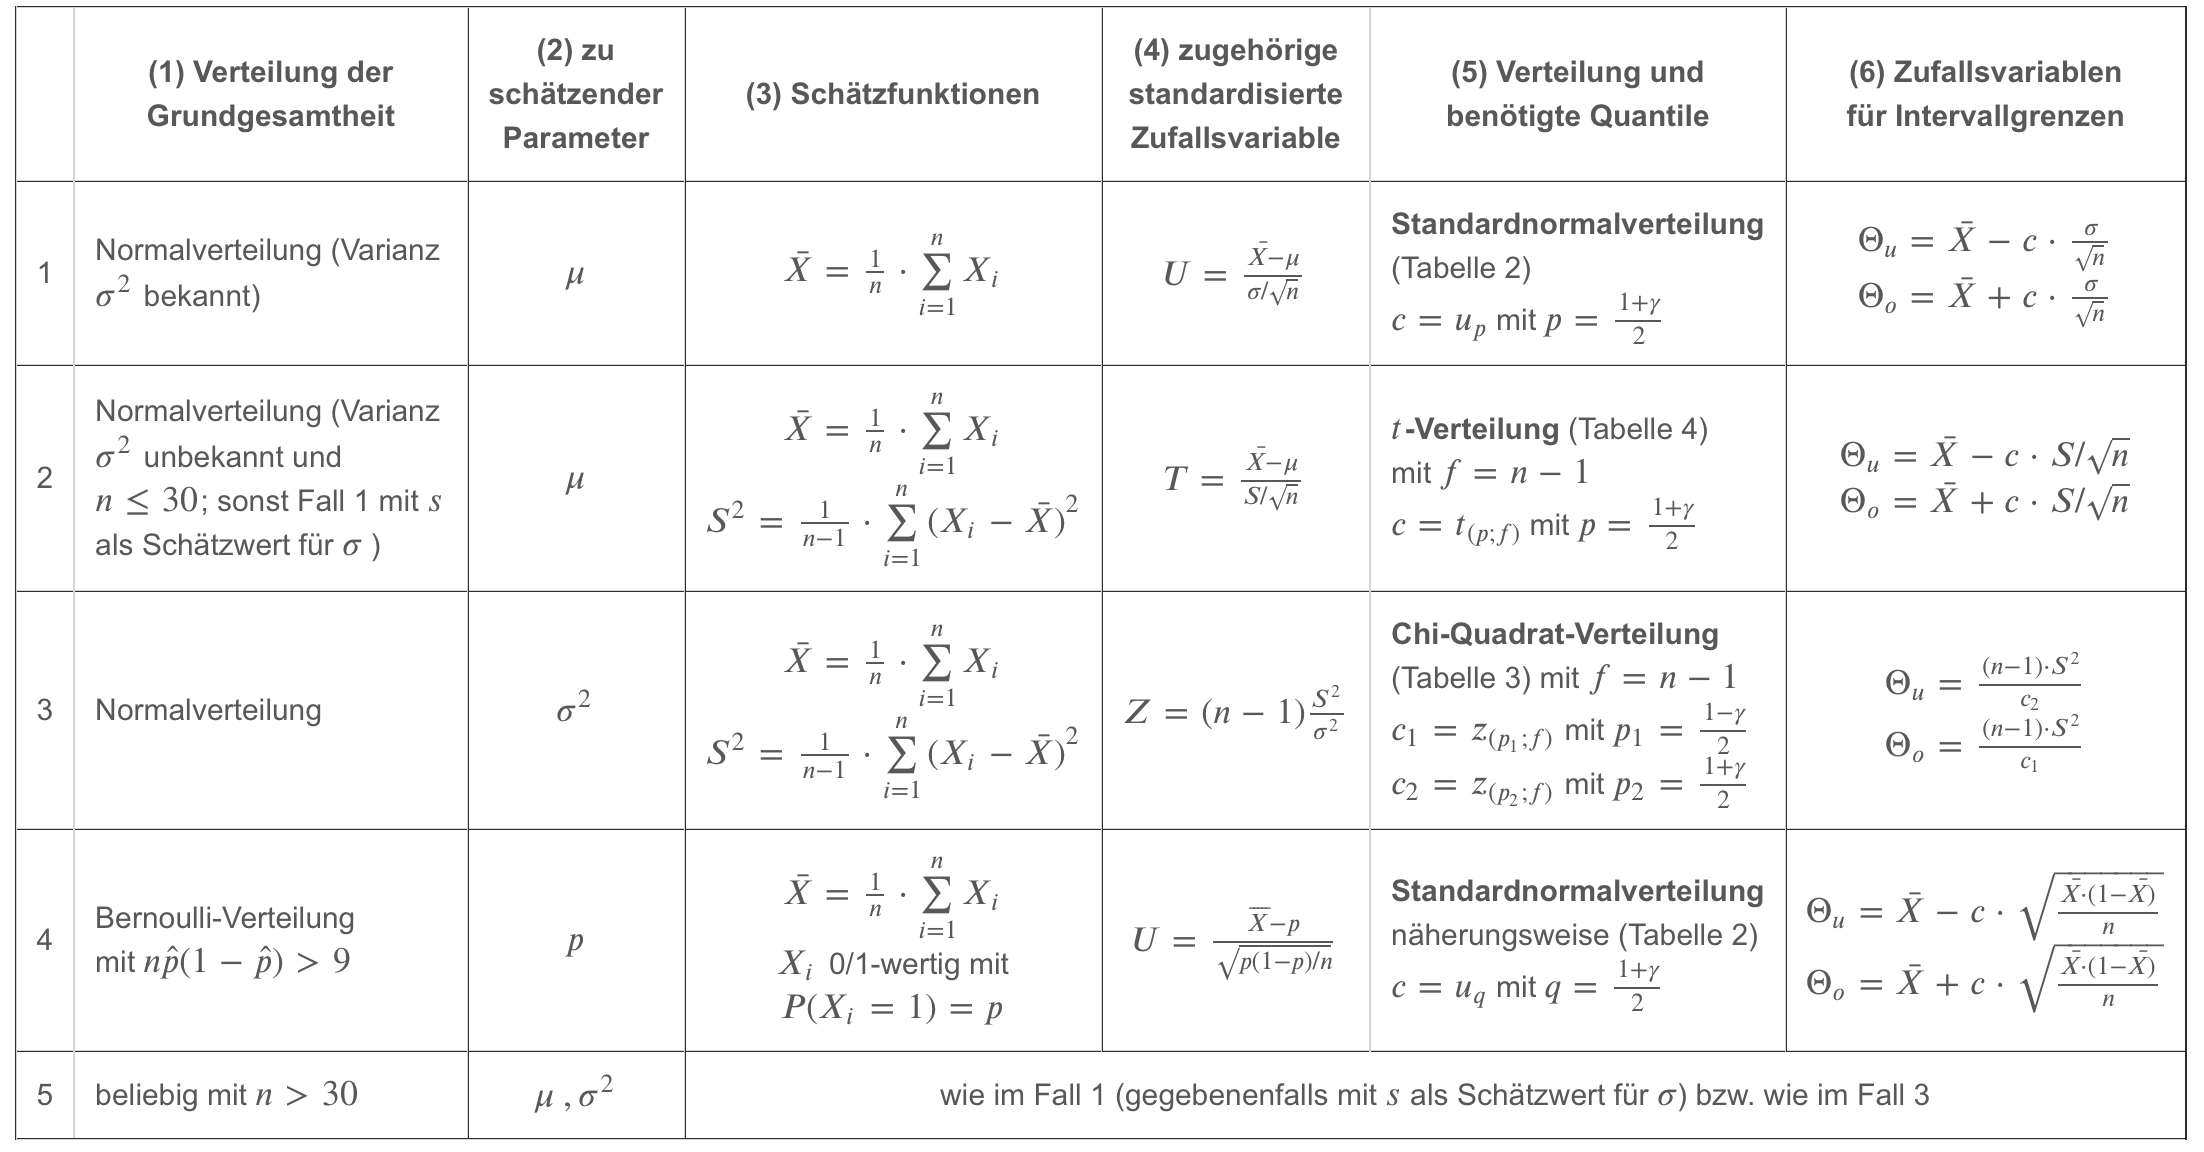
\includegraphics[width=1\linewidth]{images/vertrauensintervalle}
\end{center}
\subsection{Hypothesentests}
\label{sec:hypothesentests}
\subsubsection{Vorgehen bei einem Parametertest}
\label{sec:vorgehen_bei_einem_parametertest}
\begin{center}
    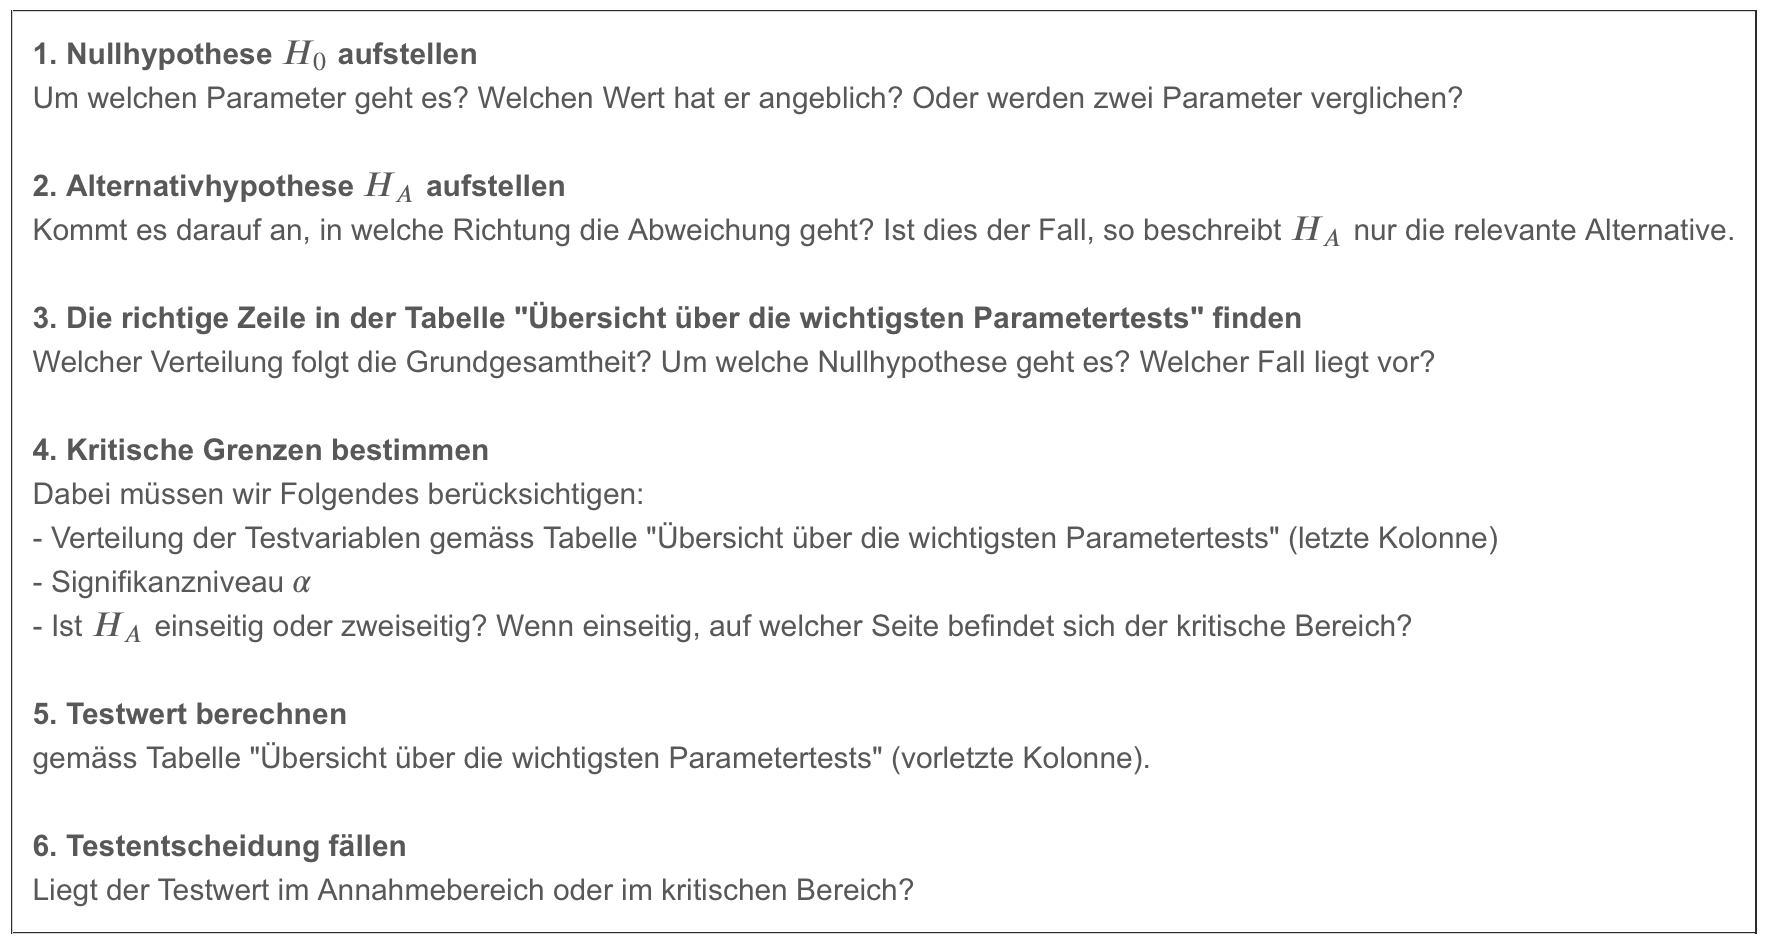
\includegraphics[width=1\linewidth]{images/parametertests}
\end{center}
\subsubsection{Übersicht über die wichtigsten Parametertests}
\label{sec:uebersicht_ueber_die_wichtigsten_parametertests}
\begin{center}
    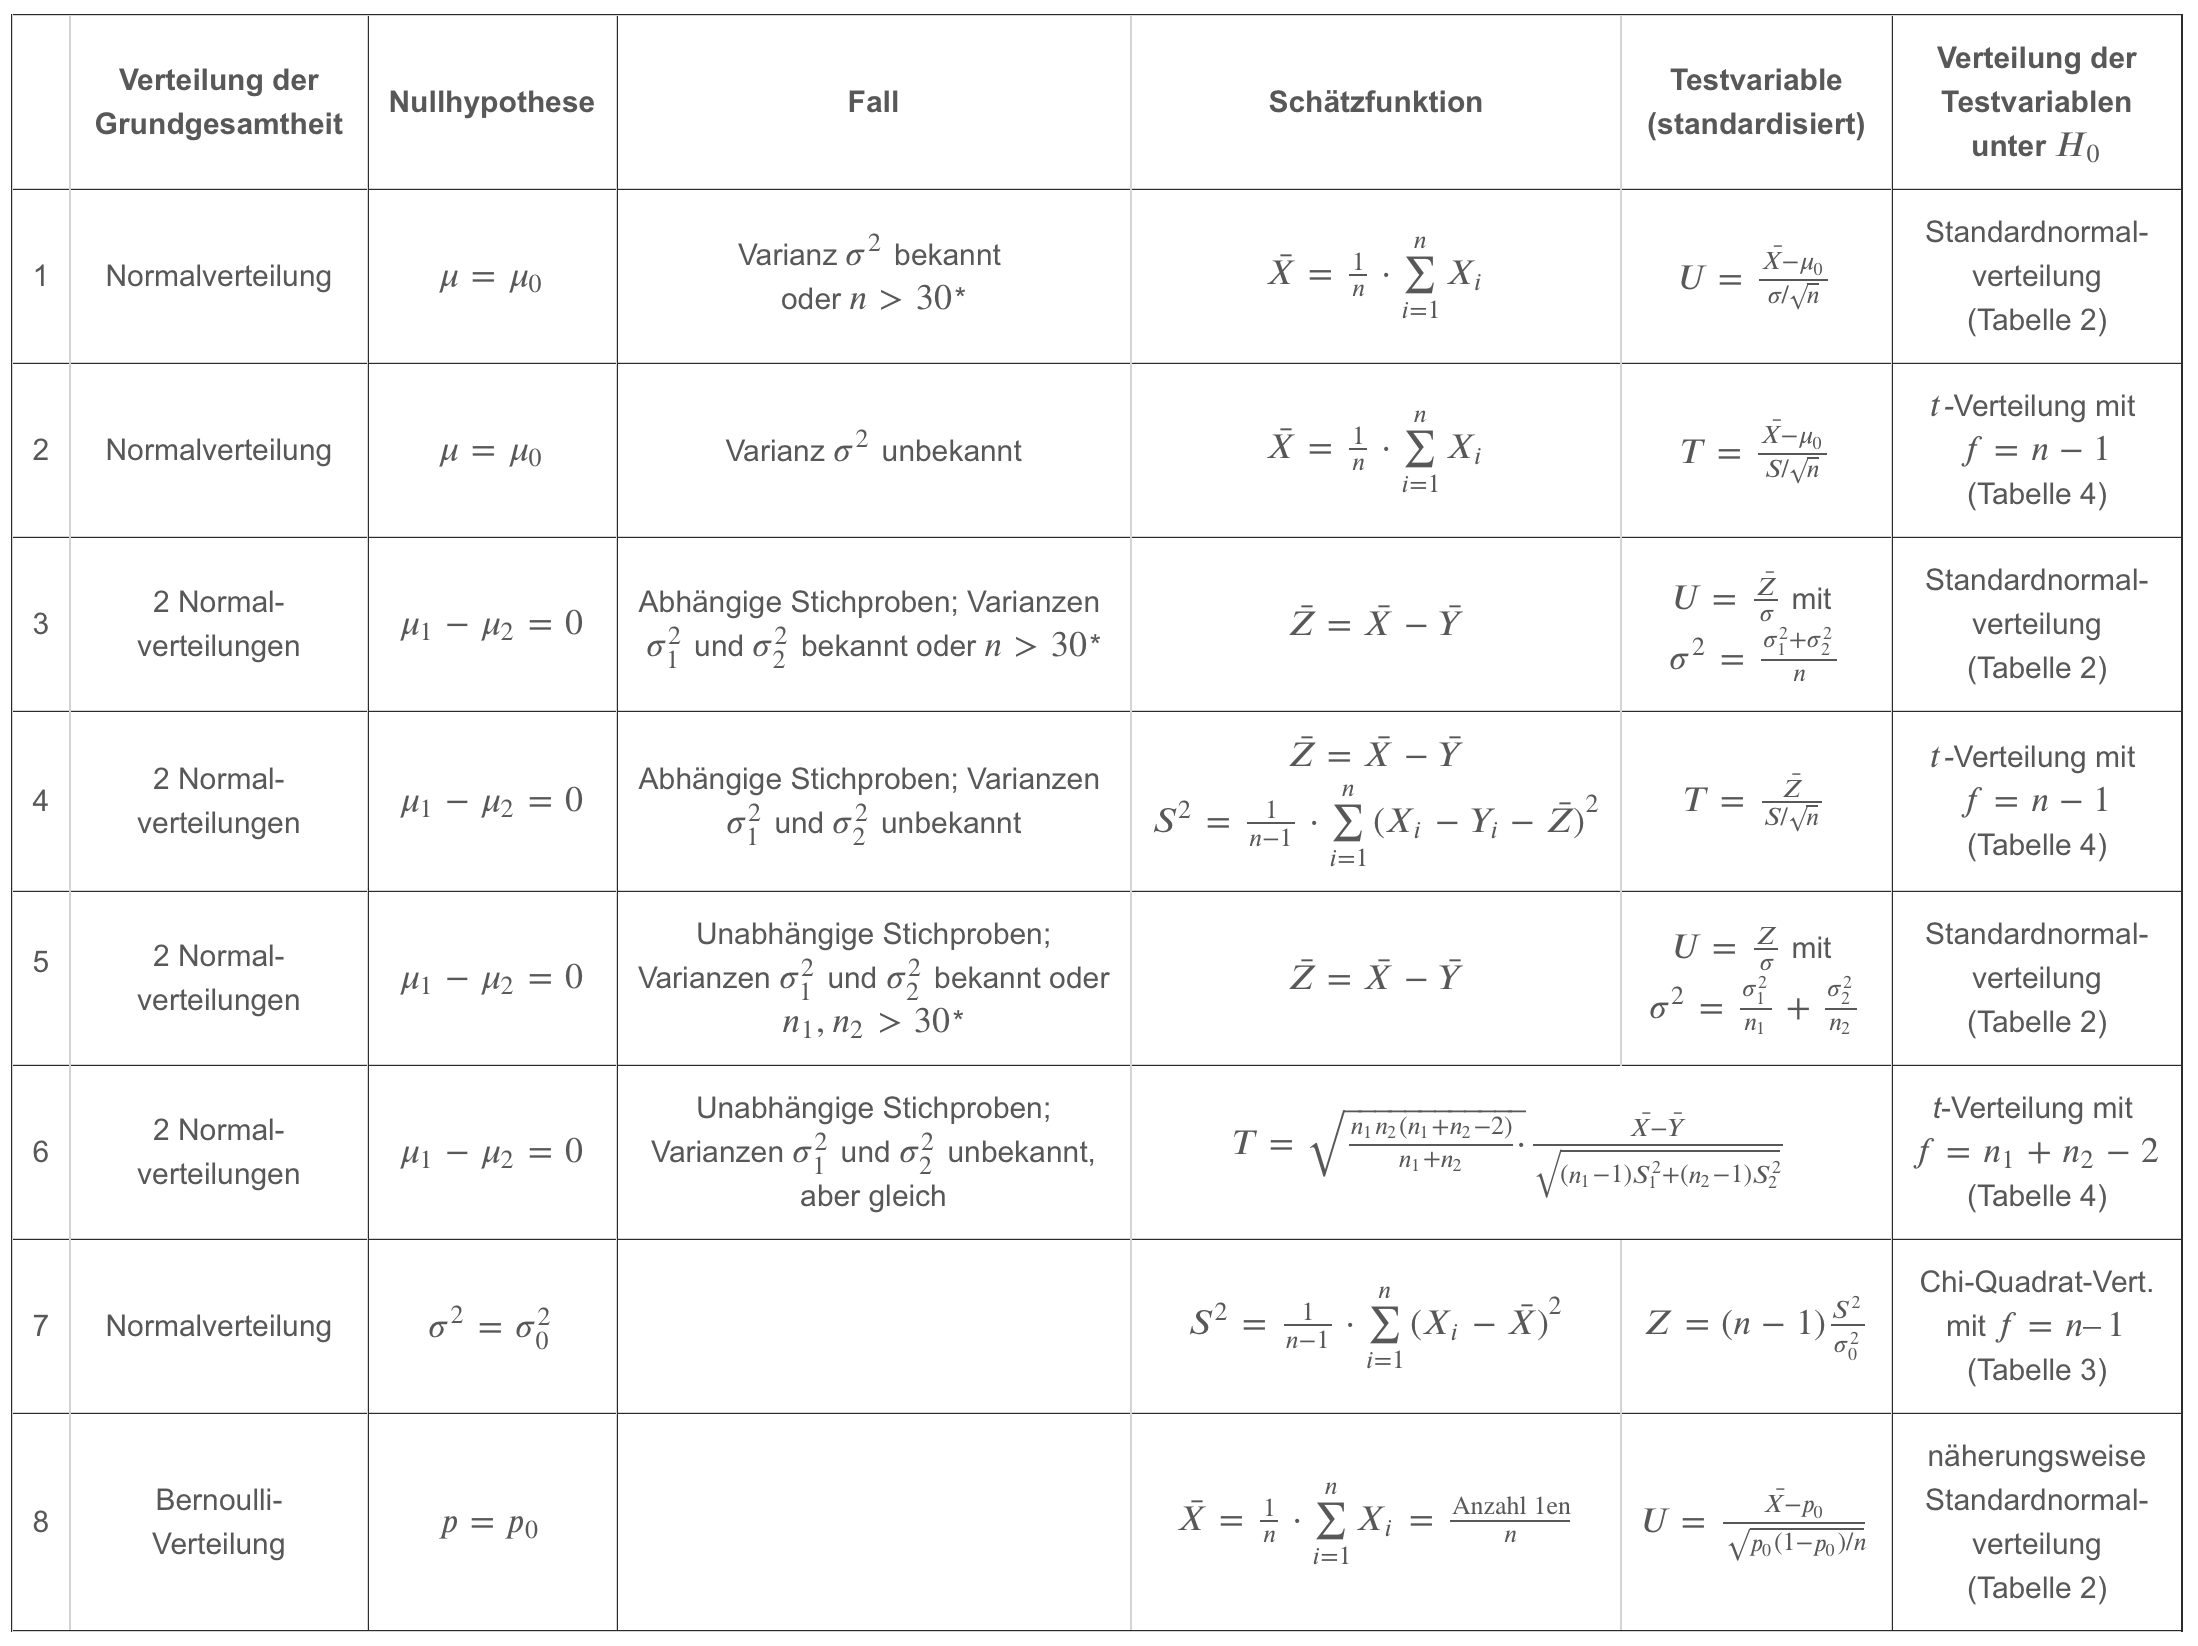
\includegraphics[width=1\linewidth]{images/parametertests2}
\end{center}
*) falls gilt: $n > 30$ bzw. $n_1 > 30$ und $n_2 > 30$, so kann der entsprechende Fall für bekannte Varianzen angewendet werden; dabei dient $s$ als
Schätzwert für $\sigma$ bzw. $s_i$ als Schätzwert für $\sigma_i$.
\subsubsection{Mögliche Fehler bei einem Hypothesentest}
\label{sec:moegliche_fehler_bei_einem_hypothesentest}
\begin{center}
    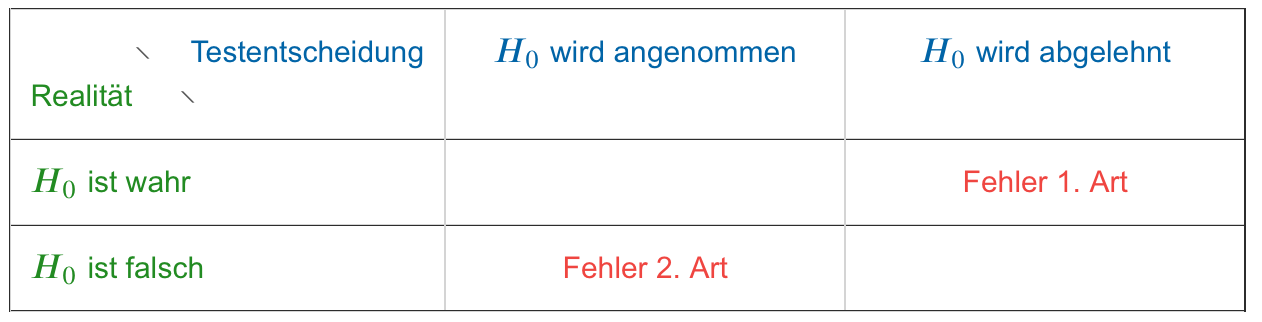
\includegraphics[width=1\linewidth]{images/fehler}
\end{center}
\subsubsection{Der p-Wert}
\label{sec:der_p-wert}
Der p-Wert ist die Wahrscheinlichkeit, dass die Testvariable $T$ einen Wert annimmt, der mindestens so extrem ist wie der Testwert $\hat{t}$, 
der aufgrund der Stichprobe berechnet wurde, wenn $H_0$ wahr ist.
\begin{center}
    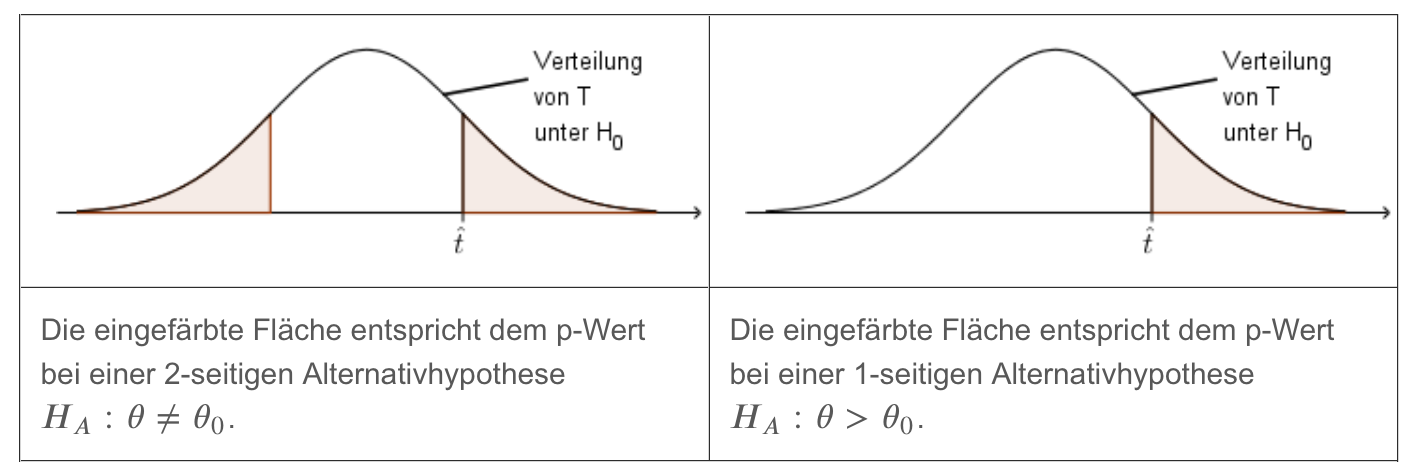
\includegraphics[width=1\linewidth]{images/p-wert}
\end{center}